\documentclass{article}

\usepackage{graphicx}

\usepackage{amsfonts, amsmath, amssymb, amsthm}
\usepackage{bigfoot}
\usepackage{comment}
\usepackage[shortlabels]{enumitem}
\usepackage{etoolbox}
\usepackage{environ}
\usepackage{fontawesome5}
\usepackage{mathabx, mathrsfs}
\usepackage{soul}
\usepackage{stmaryrd}
% Must load `xcolor` before `tcolorbox` and `tikz`.
\usepackage[dvipsnames]{xcolor}
\usepackage{tcolorbox}
\usepackage{tikz}
% `hyperref` comes after `xr-hyper`.
\usepackage{xr-hyper}
\usepackage{hyperref}

% Open "private" namespace.
\makeatletter

% ========================================
% General
% ========================================

\newcommand{\header}[2]{\title{#1}\author{#2}\date{}\maketitle}

% ========================================
% Dividers
% ========================================

\newcommand\@linespace{\vspace{10pt}}
\newcommand\linedivider{\@linespace\hrule\@linespace}
\WithSuffix\newcommand\linedivider*{\@linespace\hrule}
\newcommand\suitdivider{$$\spadesuit\;\spadesuit\;\spadesuit$$}

% ========================================
% Linking
% ========================================

\hypersetup{colorlinks=true, linkcolor=blue, urlcolor=blue}
\newcommand{\textref}[1]{\text{\nameref{#1}}}
\newcommand{\hyperlabel}[1]{%
  \label{#1}%
  \hypertarget{#1}{}}

% Links to theorems/statements/etc. that can be found in Mathlib4's index.
\newcommand\@leanlink[3]{%
  \textcolor{BlueViolet}{\raisebox{-4.5pt}{%
    \tikz{\draw (0, 0) node[yscale=-1,xscale=1] {\faFont};}}{-\;}}%
  \href{https://leanprover-community.github.io/mathlib4_docs/#1.html\##2}%
  {\color{BlueViolet}{#3}}}

\newcommand\lean[2]{%
  \noindent\@leanlink{#1}{#2}{#2}}
\WithSuffix\newcommand\lean*[2]{%
  \vspace{6pt}\lean{#1}{#2}}

\newcommand\leanp[3]{%
  \noindent\@leanlink{#1}{#2}{#3}}
\WithSuffix\newcommand\leanp*[3]{%
  \vspace{6pt}\leanp{#1}{#2}{#3}}

% Links to theorems/statements/etc. found in custom index.
\newcommand\@codelink[4]{%
  \textcolor{MidnightBlue}{\raisebox{-4.5pt}{%
    \tikz{\draw (0, 0) node[xshift=8pt] {\faCodeBranch};}}{-\;}}%
  \href{#1/#2.html\##3}%
  {\color{MidnightBlue}{#4}}}

\newcommand\coderef[3]{%
  \@codelink{#1}{#2}{#3}{#3}}
\newcommand\codepref[4]{%
  \@codelink{#1}{#2}{#3}{#4}}

% Macro to build our `code` commands relative to a given directory. For
% instance, we expect to have invocation `\makecode{..}` if the TeX file exists
% one directory deep from the root of our project..
\newcommand\makecode[1]{%
  \newcommand\code[2]{%
    \noindent\coderef{#1}{##1}{##2}}
  \WithSuffix\newcommand\code*[2]{%
    \vspace{6pt}\noindent\coderef{#1}{##1}{##2}}

  \newcommand\codep[3]{%
    \noindent\codepref{#1}{##1}{##2}{##3}}
  \WithSuffix\newcommand\codep*[3]{%
    \vspace{6pt}\noindent\codepref{#1}{##1}{##2}{##3}}
}

% ========================================
% Admonitions
% ========================================

\NewEnviron{note}{%
  \begin{tcolorbox}[%
      sharp corners,
      fonttitle=\sffamily\bfseries,
      toptitle=2pt,
      bottomtitle=2pt,
      coltitle=black!80!white,
      colback=yellow!30,
      colframe=yellow!80!black,
      title=Note]
    \BODY
  \end{tcolorbox}}

% ========================================
% Statements
% ========================================

\newcommand\@statement[1]{%
  \linedivider*\paragraph{\normalfont\normalsize\textit{#1.}}}
\newenvironment{answer}{\@statement{Answer}}{\hfill$\square$}
\renewenvironment{proof}{\@statement{Proof}}{\hfill$\square$}

\newtheorem{corollaryinner}{Corollary}
\newenvironment{corollary}[1][]{%
  \ifstrempty{#1}
    {\corollaryinner}
    {\renewcommand\thecorollaryinner{#1}\corollaryinner}
}{\endcorollaryinner}

\newtheorem{lemmainner}{Lemma}
\newenvironment{lemma}[1][]{%
  \ifstrempty{#1}
    {\lemmainner}
    {\renewcommand\thelemmainner{#1}\lemmainner}
}{\endlemmainner}

\newtheorem{theoreminner}{Theorem}
\newenvironment{theorem}[1][]{%
  \ifstrempty{#1}
    {\theoreminner}
    {\renewcommand\thetheoreminner{#1}\theoreminner}
}{\endtheoreminner}

% ========================================
% Status
% ========================================

\DeclareRobustCommand{\defined}[1]{%
  \texorpdfstring{\color{darkgray}\faParagraph\ #1}{#1}}
\DeclareRobustCommand{\verified}[1]{%
  \texorpdfstring{\color{teal}\faCheckCircle\ #1}{#1}}
\DeclareRobustCommand{\unverified}[1]{%
  \texorpdfstring{\color{olive}\faCheckCircle[regular]\ #1}{#1}}
\DeclareRobustCommand{\pending}[1]{%
  \texorpdfstring{\color{Fuchsia}\faPencil*\ #1}{#1}}
\DeclareRobustCommand{\sorry}[1]{%
  \texorpdfstring{\color{Maroon}\faExclamationCircle\ #1}{#1}}

% ========================================
% Math
% ========================================

\newcommand{\abs}[1]{\left|#1\right|}
\newcommand{\ceil}[1]{\left\lceil#1\right\rceil}
\newcommand{\dom}[1]{\textop{dom}{#1}}
\newcommand{\fld}[1]{\textop{fld}{#1}}
\newcommand{\floor}[1]{\left\lfloor#1\right\rfloor}
\newcommand{\icc}[2]{\left[#1, #2\right]}
\newcommand{\ico}[2]{\left[#1, #2\right)}
\newcommand{\img}[2]{#1\!\left\llbracket#2\right\rrbracket}
\newcommand{\ioc}[2]{\left(#1, #2\right]}
\newcommand{\ioo}[2]{\left(#1, #2\right)}
\newcommand{\powerset}[1]{\mathscr{P}#1}
\newcommand{\ran}[1]{\textop{ran}{#1}}
\newcommand{\textop}[1]{\mathop{\text{#1}}}
\newcommand{\ubar}[1]{\text{\b{$#1$}}}

\let\oldemptyset\emptyset
\let\emptyset\varnothing

% Close off "private" namespace.
\makeatother


\graphicspath{{./images/}}

\externaldocument[A:]
  {../../Common/Real/Geometry/Area}
  [../../Common/Real/Geometry/Area.pdf]

\begin{document}

\header{Exercises 1.7}{Tom M. Apostol}

The properties of area in this set of exercises are to be deduced from the
  axioms for area stated in the foregoing section.

\section*{Exercise 1}%
\label{sec:exercise-1}

Prove that each of the following sets is measurable and has zero area:

\subsection*{\proceeding{Exercise 1a}}%
\label{sub:exercise-1a}

A set consisting of a single point.

\begin{proof}

  Let $S$ be a set consisting of a single point.
  By definition of a Point, $S$ is a rectangle in which all vertices coincide.
  By \nameref{A:sec:choice-scale}, $S$ is measurable with area its width times
    its height.
  The width and height of $S$ is trivially zero.
  Therefore $a(S) = (0)(0) = 0$.

\end{proof}

\subsection*{\proceeding{Exercise 1b}}%
\label{sub:exercise-1b}

A set consisting of a finite number of points in a plane.

\begin{proof}

  Define predicate $P(n)$ as "A set consisting of $n$ points in a plane is
    measurable with area $0$".
  We use induction to prove $P(n)$ holds for all $n > 0$.

  \paragraph{Base Case}%

    Consider a set $S$ consisting of a single point in a plane.
    By \nameref{sub:exercise-1a}, $S$ is measurable with area $0$.
    Thus $P(1)$ holds.

  \paragraph{Induction Step}%

    Assume induction hypothesis $P(k)$ holds for some $k > 0$.
    Let $S_{k+1}$ be a set consisting of $k + 1$ points in a plane.
    Pick an arbitrary point of $S_{k+1}$.
    Denote the set containing just this point as $T$.
    Denote the remaining set of points as $S_k$.
    By construction, $S_{k+1} = S_k \cup T$.
    By the induction hypothesis, $S_k$ is measurable with area $0$.
    By \nameref{sub:exercise-1a}, $T$ is measurable with area $0$.
    By the \nameref{A:sec:additive-property}, $S_k \cup T$ is
      measurable, $S_k \cap T$ is measurable, and
      \begin{align}
        a(S_{k+1})
          & = a(S_k \cup T) \nonumber \\
          & = a(S_k) + a(T) - a(S_k \cap T) \nonumber \\
          & = 0 + 0 - a(S_k \cap T). \label{sub:exercise-1b-eq1}
      \end{align}
    There are two cases to consider:

    \subparagraph{Case 1}%

      $S_k \cap T = \emptyset$.
      Then it trivially follows that $a(S_k \cap T) = 0$.

    \subparagraph{Case 2}%

      $S_k \cap T \neq \emptyset$.
      Since $T$ consists of a single point, $S_k \cap T = T$.
      By \nameref{sub:exercise-1a}, $a(S_k \cap T) = a(T) = 0$.

    \vspace{8pt}
    \noindent
    In both cases, \eqref{sub:exercise-1b-eq1} evaluates to $0$, implying
      $P(k + 1)$ as expected.

  \paragraph{Conclusion}%

    By mathematical induction, it follows for all $n > 0$, $P(n)$ is true.

\end{proof}

\subsection*{\proceeding{Exercise 1c}}%
\label{sub:exercise-1c}

The union of a finite collection of line segments in a plane.

\begin{proof}

  Define predicate $P(n)$ as "A set consisting of $n$ line segments in a plane
    is measurable with area $0$".
  We use induction to prove $P(n)$ holds for all $n > 0$.

  \paragraph{Base Case}%

    Consider a set $S$ consisting of a single line segment in a plane.
    By definition of a Line Segment, $S$ is a rectangle in which one side has
      dimension $0$.
    By \nameref{A:sec:choice-scale}, $S$ is measurable with area its width $w$
      times its height $h$.
    Therefore $a(S) = wh = 0$.
    Thus $P(1)$ holds.

  \paragraph{Induction Step}%

    Assume induction hypothesis $P(k)$ holds for some $k > 0$.
    Let $S_{k+1}$ be a set consisting of $k + 1$ line segments in a plane.
    Pick an arbitrary line segment of $S_{k+1}$.
    Denote the set containing just this line segment as $T$.
    Denote the remaining set of line segments as $S_k$.
    By construction, $S_{k+1} = S_k \cup T$.
    By the induction hypothesis, $S_k$ is measurable with area $0$.
    By the base case, $T$ is measurable with area $0$.
    By the \nameref{A:sec:additive-property}, $S_k \cup T$ is measurable,
      $S_k \cap T$ is measurable, and
      \begin{align}
        a(S_{k+1})
          & = a(S_k \cup T) \nonumber \\
          & = a(S_k) + a(T) - a(S_k \cap T) \nonumber \\
          & = 0 + 0 - a(S_k \cap T). \label{sub:exercise-1c-eq1}
      \end{align}
    There are two cases to consider:

    \subparagraph{Case 1}%

      $S_k \cap T = \emptyset$.
      Then it trivially follows that $a(S_k \cap T) = 0$.

    \subparagraph{Case 2}%

      $S_k \cap T \neq \emptyset$.
      Since $T$ consists of a single point, $S_k \cap T = T$.
      By the base case, $a(S_k \cap T) = a(T) = 0$.

    \vspace{8pt}
    \noindent
    In both cases, \eqref{sub:exercise-1c-eq1} evaluates to $0$, implying
      $P(k + 1)$ as expected.

  \paragraph{Conclusion}%

    By mathematical induction, it follows for all $n > 0$, $P(n)$ is true.

\end{proof}

\section*{\unverified{Exercise 2}}%
\label{sec:exercise-2}

Every right triangular region is measurable because it can be obtained as the
  intersection of two rectangles.
Prove that every triangular region is measurable and that its area is one half
  the product of its base and altitude.

\begin{proof}

  Let $T'$ be a triangular region with base of length $a$, height of length $b$,
    and hypotenuse of length $c$.
  Consider the translation and rotation of $T'$, say $T$, such that its
    hypotenuse is entirely within quadrant I and the vertex opposite the
    hypotenuse is situated at point $(0, 0)$.

  Let $R$ be a rectangle of width $a$, height $b$, and bottom-left corner at
    $(0, 0)$.
  By construction, $R$ covers all of $T$.
  Let $S$ be a rectangle of width $c$ and height $a\sin{\theta}$, where $\theta$
    is the acute angle measured from the bottom-right corner of $T$ relative
    to the $x$-axis.
  As an example, consider the image below of triangle $T$ with width $4$ and
    height $3$:

  \begin{figure}[h]
    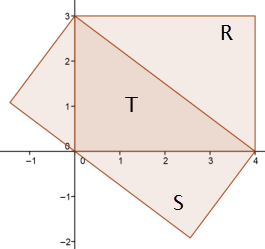
\includegraphics{right-triangle}
    \centering
  \end{figure}

  By \nameref{A:sec:choice-scale}, both $R$ and $S$ are measurable.
  By this same axiom, $a(R) = ab$ and $a(S) = ca\sin{\theta}$.
  By the \nameref{A:sec:additive-property}, $R \cup S$ and $R \cap S$ are both
    measurable.
  $a(R \cap S) = a(T)$ and $a(R \cup S)$ can be determined by noting that
    $R$'s construction implies identity $a(R) = 2a(T)$.
  Therefore
    \begin{align*}
      a(T)
        & = a(R \cap S) \\
        & = a(R) + a(S) - a(R \cup S) \\
        & = ab + ca\sin{\theta} - a(R \cup S) \\
        & = ab + ca\sin{\theta} - (ca\sin{\theta} + \frac{1}{2}a(R)) \\
        & = ab + ca\sin{\theta} - ca\sin{\theta} - a(T).
    \end{align*}
  Solving for $a(T)$ gives the desired identity: $$a(T) = \frac{1}{2}ab.$$
  By \nameref{A:sec:invariance-under-congruence}, $a(T') = a(T)$, concluding our
    proof.

\end{proof}

\section*{\unverified{Exercise 3}}%
\label{sec:exercise-3}

Prove that every trapezoid and every parallelogram is measurable and derive the
  usual formulas for their areas.

\begin{proof}

  We begin by proving the formula for a trapezoid.
  Let $S$ be a trapezoid with height $h$ and bases $b_1$ and $b_2$, $b_1 < b_2$.
  There are three cases to consider:

  \begin{figure}[h]
    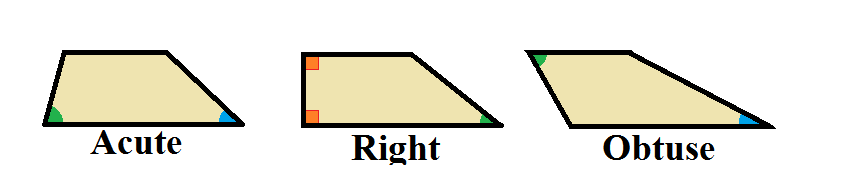
\includegraphics[width=\textwidth]{trapezoid-cases}
    \centering
  \end{figure}

  \paragraph{Case 1}%

    Suppose $S$ is a right trapezoid.
    Then $S$ is the union of non-overlapping rectangle $R$ of width $b_1$ and
      height $h$ with right triangle $T$ of base $b_2 - b_1$ and height $h$.
    By \nameref{A:sec:choice-scale}, $R$ is measurable.
    By \nameref{sec:exercise-2}, $T$ is measurable.
    By the \nameref{A:sec:additive-property}, $R \cup T$ and $R \cap T$ are both
      measurable and
      \begin{align*}
        a(S)
          & = a(R \cup T) \\
          & = a(R) + a(T) - a(R \cap T) \\
          & = a(R) + a(T) & \text{by construction} \\
          & = b_1h + a(T) & \text{Choice of Scale} \\
          & = b_1h + \frac{1}{2}(b_2 - b_1)h
            & \text{\nameref{sec:exercise-2}} \\
          & = \frac{b_1 + b_2}{2}h.
      \end{align*}

  \paragraph{Case 2}%

    Suppose $S$ is an acute trapezoid.
    Then $S$ is the union of non-overlapping triangle $T$ and right trapezoid $R$.
    Let $c$ denote the length of base $T$.
    Then $R$ has longer base edge of length $b_2 - c$.
    By \nameref{sec:exercise-2}, $T$ is measurable.
    By Case 1, $R$ is measurable.
    By the \nameref{A:sec:additive-property}, $R \cup T$ and $R \cap T$ are both
      measurable and
      \begin{align*}
        a(S)
          & = a(T) + a(R) - a(R \cap T) \\
          & = a(T) + a(R) & \text{by construction} \\
          & = \frac{1}{2}ch + a(R) & \text{\nameref{sec:exercise-2}} \\
          & = \frac{1}{2}ch + \frac{b_1 + b_2 - c}{2}h & \text{Case 1} \\
          & = \frac{b_1 + b_2}{2}h.
      \end{align*}

  \paragraph{Case 3}%

    Suppose $S$ is an obtuse trapezoid.
    Then $S$ is the union of non-overlapping triangle $T$ and right trapezoid $R$.
    Let $c$ denote the length of base $T$.
    Reflect $T$ vertically to form another right triangle, say $T'$.
    Then $T' \cup R$ is an acute trapezoid.
    By \nameref{A:sec:invariance-under-congruence},
      \begin{equation}
        \label{par:exercise-3-case-3-eq1}
        \tag{3.1}
        a(T' \cup R) = a(T \cup R).
      \end{equation}
    By construction, $T' \cup R$ has height $h$ and bases $b_1 - c$ and $b_2 + c$
      meaning
      \begin{align*}
        a(T \cup R)
          & = a(T' \cup R) & \eqref{par:exercise-3-case-3-eq1} \\
          & = \frac{b_1 - c + b_2 + c}{2}h & \text{Case 2} \\
          & = \frac{b_1 + b_2}{2}h.
      \end{align*}

  \paragraph{Conclusion}%

    These cases are exhaustive and in agreement with one another.
    Thus $S$ is measurable and $$a(S) = \frac{b_1 + b_2}{2}h.$$

  \divider

  Let $P$ be a parallelogram with base $b$ and height $h$.
  Then $P$ is the union of non-overlapping triangle $T$ and right trapezoid $R$.
  Let $c$ denote the length of base $T$.
  Reflect $T$ vertically to form another right triangle, say $T'$.
  Then $T' \cup R$ is an acute trapezoid.
  By \nameref{A:sec:invariance-under-congruence},
    \begin{equation}
      \label{par:exercise-3-eq2}
      \tag{3.2}
      a(T' \cup R) = a(T \cup R).
    \end{equation}
  By construction, $T' \cup R$ has height $h$ and bases $b - c$ and $b + c$
    meaning
    \begin{align*}
      a(T \cup R)
        & = a(T' \cup R) & \eqref{par:exercise-3-eq2} \\
        & = \frac{b - c + b + c}{2}h & \text{Area of Trapezoid} \\
        & = bh.
    \end{align*}

\end{proof}

\section*{Exercise 4}%
\label{sec:exercise-4}

Let $P$ be a polygon whose vertices are lattice points.
The area of $P$ is $I + \frac{1}{2}B - 1$, where $I$ denotes the number of
  lattice points inside the polygon and $B$ denotes the number on the boundary.

\subsection*{\unverified{Exercise 4a}}%
\label{sub:exercise-4a}

Prove that the formula is valid for rectangles with sides parallel to the
  coordinate axes.

\begin{proof}

  Let $P$ be a rectangle with sides parallel to the coordinate axes, with width
    $w$, height $h$, and lattice points for vertices.
  We assume $P$ has three non-collinear points, ruling out any instances of
    points or line segments.

  By \nameref{A:sec:choice-scale}, $P$ is measurable with area $a(P) = wh$.
  By construction, $P$ has $I = (w - 1)(h - 1)$ interior lattice points and
    $B = 2(w + h)$ lattice points on its boundary.
  The following shows the lattice point area formula is in agreement with
    the expected result:
    \begin{align*}
      I + \frac{1}{2}B - 1
        & = (w - 1)(h - 1) + \frac{1}{2}\left[ 2(w + h) \right] - 1 \\
        & = (wh - w - h + 1) + \frac{1}{2}\left[ 2(w + h) \right] - 1 \\
        & = (wh - w - h + 1) + (w + h) - 1 \\
        & = wh.
    \end{align*}

\end{proof}

\subsection*{\unverified{Exercise 4b}}%
\label{sub:exercise-4b}

Prove that the formula is valid for right triangles and parallelograms.

\begin{proof}

  Let $P$ be a right triangle with width $w > 0$, height $h > 0$, and lattice
    points for vertices.
  Let $T$ be the triangle $P$ translated, rotated, and reflected such that the
    its vertices are $(0, 0)$, $(0, w)$, and $(w, h)$.
  Let $I_T$ and $B_T$ be the number of interior and boundary points of $T$
    respectively.
  Let $H_L$ denote the number of lattice points on $T$'s hypotenuse.

  Let $R$ be the overlapping rectangle of width $w$ and height $h$, situated
    with bottom-left corner at $(0, 0)$.
  Let $I_R$ and $B_R$ be the number of interior and boundary points
    of $R$ respectively.

  By construction, $T$ shares two sides with $R$.
  Therefore
    \begin{equation}
      \label{sub:exercise-4b-eq1}
      B_T = \frac{1}{2}B_R - 1 + H_L.
    \end{equation}
  Likewise,
    \begin{equation}
      \label{sub:exercise-4b-eq2}
      I_T = \frac{1}{2}(I_R - H_L + 2).
    \end{equation}
  The following shows the lattice point area formula is in agreement with
    the expected result:
    \begin{align*}
      I_T + \frac{1}{2}B_T - 1
        & = \frac{1}{2}(I_R - H_L + 2) + \frac{1}{2}B_T - 1
          & \eqref{sub:exercise-4b-eq2} \\
        & = \frac{1}{2}\left[ I_R - H_L + 2 + B_T - 2 \right] \\
        & = \frac{1}{2}\left[ I_R - H_L + B_T \right] \\
        & = \frac{1}{2}\left[ I_R - H_L + \frac{1}{2}B_R - 1 + H_L \right]
          & \eqref{sub:exercise-4b-eq1} \\
        & = \frac{1}{2}\left[ I_R + \frac{1}{2}B_R - 1 \right] \\
        & = \frac{1}{2}\left[ (w - 1)(h - 1) + \frac{1}{2}(2(w + h)) - 1 \right]
          & \text{\nameref{sub:exercise-4a}} \\
        & = \frac{1}{2}\left[ (w - 1)(h - 1) + w + h - 1 \right] \\
        & = \frac{1}{2}\left[ wh - w - h + 1 + w + h - 1 \right] \\
        & = \frac{wh}{2}.
    \end{align*}

  We do not prove this formula is valid for parallelograms here.
  Instead, refer to \nameref{sub:exercise-4c} below.

\end{proof}

\subsection*{\unverified{Exercise 4c}}%
\label{sub:exercise-4c}

Use induction on the number of edges to construct a proof for general polygons.

\begin{proof}

  Define predicate $P(n)$ as "An $n$-polygon with vertices on lattice points has
    area $I + \frac{1}{2}B - 1$."
  We use induction to prove $P(n)$ holds for all $n \geq 3$.

  \paragraph{Base Case}%

    A $3$-polygon is a triangle.
    By \nameref{sub:exercise-4b}, the lattice point area formula holds.
    Thus $P(3)$ holds.

  \paragraph{Induction Step}%

    Assume induction hypothesis $P(k)$ holds for some $k \geq 3$.
    Let $P$ be a $(k + 1)$-polygon with vertices on lattice points.
    Such a polygon is equivalent to the union of a $k$-polygon $S$ with a
      triangle $T$.
    That is, $P = S \cup T$.

    Let $I_P$ be the number of interior lattice points of $P$.
    Let $B_P$ be the number of boundary lattice points of $P$.
    Similarly, let $I_S$, $I_T$, $B_S$, and $B_T$ be the number of interior
      and boundary lattice points of $S$ and $T$.
    Let $c$ denote the number of boundary points shared between $S$ and $T$.

    By our induction hypothesis, $a(S) = I_S + \frac{1}{2}B_S - 1$.
    By our base case, $a(T) = I_T + \frac{1}{2}B_T - 1$.
    By construction, it follows:
      \begin{align*}
        I_P & = I_S + I_T + c - 2 \\
        B_P & = B_S + B_T - (c - 2) - c \\
            & = B_S + B_T - 2c + 2.
      \end{align*}
    Applying the lattice point area formula to $P$ yields the following:
      \begin{align*}
        & I_P + \frac{1}{2}B_P - 1 \\
          & = (I_S + I_T + c - 2) + \frac{1}{2}(B_S + B_T - 2c + 2) - 1 \\
          & = I_S + I_T + c - 2 + \frac{1}{2}B_S + \frac{1}{2}B_T - c + 1 - 1 \\
          & = (I_S + \frac{1}{2}B_S - 1) + (I_T + \frac{1}{2}B_T - 1) \\
          & = a(S) + (I_T + \frac{1}{2}B_T - 1) & \text{induction hypothesis} \\
          & = a(S) + a(T). & \text{base case}
      \end{align*}
    By the \nameref{A:sec:additive-property}, $S \cup T$ is measurable,
      $S \cap T$ is measurable, and
      \begin{align*}
        a(P)
          & = a(S \cup T) \\
          & = a(S) + a(T) - a(S \cap T) \\
          & = a(S) + a(T). & \text{by construction}
      \end{align*}
    This shows the lattice point area formula is in agreement with our axiomatic
      definition of area.
    Thus $P(k + 1)$ holds.

  \paragraph{Conclusion}%

    By mathematical induction, it follows for all $n \geq 3$, $P(n)$ is true.

\end{proof}

\section*{\unverified{Exercise 5}}%
\label{sec:exercise-5}

Prove that a triangle whose vertices are lattice points cannot be equilateral.

[\textit{Hint:} Assume there is such a triangle and compute its area in two
ways, using Exercises 2 and 4.]

\begin{proof}

  Proceed by contradiction.
  Let $T$ be an equilateral triangle whose vertices are lattice points.
  Assume each side of $T$ has length $a$.
  Then $T$ has height $h = (a\sqrt{3}) / 2$.
  By \nameref{sec:exercise-2},
    \begin{equation}
      \label{sub:exercise-5-eq1}
      \tag{5.1}
      a(T) = \frac{1}{2}ah = \frac{a^2\sqrt{3}}{4}.
    \end{equation}
  Let $I$ and $B$ denote the number of interior and boundary lattice points of
    $T$ respectively.
  By \nameref{sec:exercise-4},
    \begin{equation}
      \label{sub:exercise-5-eq2}
      \tag{5.2}
      a(T) = I + \frac{1}{2}B - 1.
    \end{equation}
  But \eqref{sub:exercise-5-eq1} is irrational whereas
    \eqref{sub:exercise-5-eq2} is not.
  This is a contradiction.
  Thus, there is \textit{no} equilateral triangle whose vertices are lattice
    points.

\end{proof}

\section*{\unverified{Exercise 6}}%
\label{sec:exercise-6}

Let $A = \{1, 2, 3, 4, 5\}$, and let $\mathscr{M}$ denote the class of all
  subsets of $A$.
(There are 32 altogether, counting $A$ itself and the empty set $\emptyset$.)
For each set $S$ in $\mathscr{M}$, let $n(S)$ denote the number of distinct
  elements in $S$.
If $S = \{1, 2, 3, 4\}$ and $T = \{3, 4, 5\}$, compute $n(S \cup T)$,
  $n(S \cap T)$, $n(S - T)$, and $n(T - S)$.
Prove that the set function $n$ satisfies the first three axioms for area.

\begin{proof}

  Let $S = \{1, 2, 3, 4\}$ and $T = \{3, 4, 5\}$.
  Then
    \begin{align*}
      n(S \cup T)
        & = n(\{1, 2, 3, 4\} \cup \{3, 4, 5\}) \\
        & = n(\{1, 2, 3, 4, 5\}) \\
        & = 5. \\
      n(S \cap T)
        & = n(\{1, 2, 3, 4\} \cap \{3, 4, 5\}) \\
        & = n(\{3, 4\}) \\
        & = 2. \\
      n(S - T)
        & = n(\{1, 2, 3, 4\} - \{3, 4, 5\}) \\
        & = n(\{1, 2\}) \\
        & = 2. \\
      n(T - S)
        & = n(\{3, 4, 5\} - \{1, 2, 3, 4\}) \\
        & = n(\{5\}) \\
        & = 1.
    \end{align*}
  We now prove $n$ satisfies the first three axioms for area.

  \paragraph{Nonnegative Property}%

    $n$ returns the length of some member of $\mathscr{M}$.
    By hypothesis, the smallest possible input to $n$ is $\emptyset$.
    Since $n(\emptyset) = 0$, it follows $n(S) \geq 0$ for all $S \subset A$.

  \paragraph{Additive Property}%

    Let $S$ and $T$ be members of $\mathscr{M}$.
    It trivially follows that both $S \cup T$ and $S \cap T$ are in
      $\mathscr{M}$.
    Consider the value of $n(S \cup T)$.
    There are two cases to consider:

    \subparagraph{Case 1}%

      Suppose $S \cap T = \emptyset$.
      That is, there is no common element shared between $S$ and $T$.
      Thus
        \begin{align*}
          n(S \cup T)
            & = n(S) + n(T) \\
            & = n(S) + n(T) - 0 \\
            & = n(S) + n(T) - n(S \cap T).
        \end{align*}

    \subparagraph{Case 2}%

      Suppose $S \cap T \neq \emptyset$.
      Then $n(S) + n(T)$ counts each element of $S \cap T$ twice.
      Therefore $n(S \cup T) = n(S) + n(T) - n(S \cap T)$.

    \subparagraph{Conclusion}%

      These cases are exhaustive and in agreement with one another.
      Thus $n(S \cup T) = n(S) + n(T) - n(S \cap T)$.

  \paragraph{Difference Property}%

    Suppose $S, T \in \mathscr{M}$ such that $S \subseteq T$.
    That is, every member of $S$ is a member of $T$.
    By definition, $T - S$ consists of members in $T$ but not in $S$.
    Thus $n(T - S) = n(T) - n(S)$.

\end{proof}

\end{document}
